% 2 国内外现状 或 相关研发情况
% (该部分的书写内容及标题等根据情况确定,或者删除该部分内容)
\section{相关研发情况}
\subsection{Geaflow整体架构}
GeaFlow 整体架构如下所示:
\begin{figure}[H]
  \begin{center}
    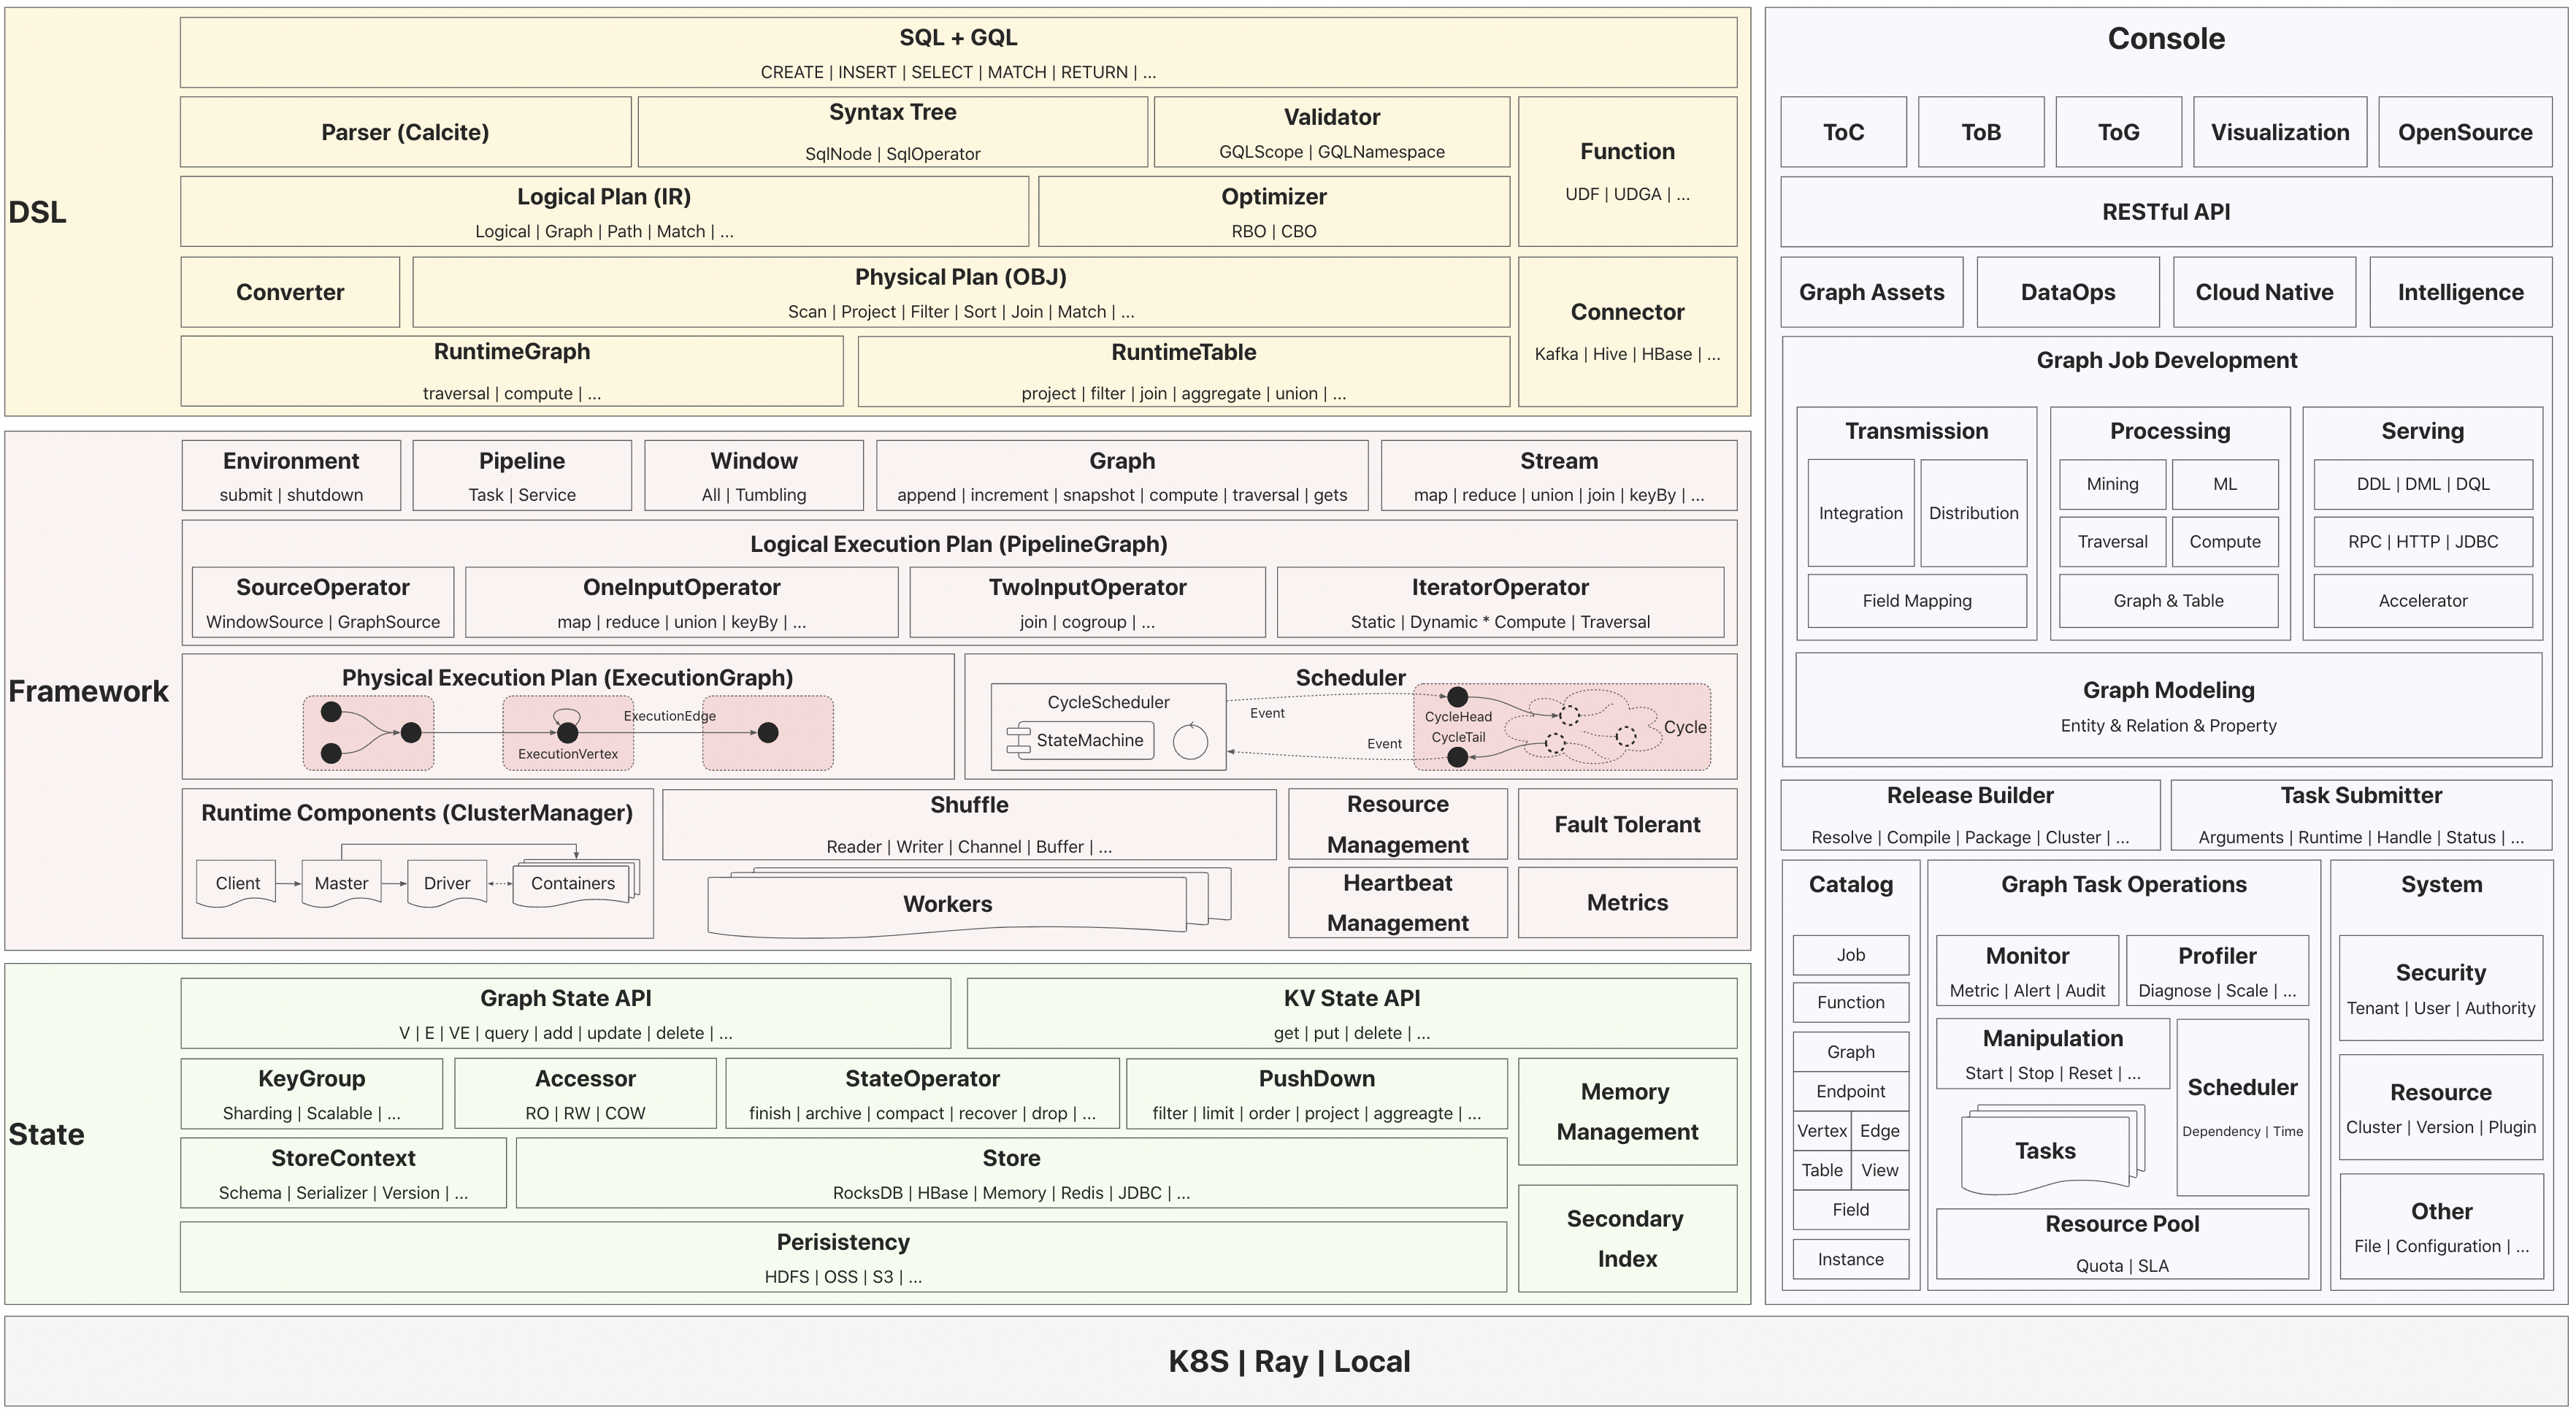
\includegraphics[width=0.95\textwidth]{./figures/geaflow_arch_new.png}
  \end{center}
  \caption{Geaflow 技术架构}
\end{figure}

\begin{itemize}
  \item DSL层:即语言层。GeaFlow设计了SQL+GQL的融合分析语言,支持对表模型和图模型统一处理。
  \item Framework层:即框架层。GeaFlow设计了面向Graph和Stream的两套API支持流、批、图融合计算,并实现了基于Cycle的统一分布式调度模型。
  \item State层:即存储层。GeaFlow设计了面向Graph和KV的两套API支持表数据和图数据的混合存储,整体采用了Sharing Nothing的设计,并支持将数据持久化到远程存储。
  \item Console平台:GeaFlow提供了一站式图研发平台,实现了图数据的建模、加工、分析能力,并提供了图作业的运维管控支持。
  \item 执行环境:GeaFlow可以运行在多种异构执行环境,如K8S、Ray以及本地模式。
\end{itemize}

\subsection{GeaFlow API 介绍}
GeaFlow API是对高阶用户提供的开发接口,其支持Graph API和Stream API两种类型:
\begin{figure}[H]
  \begin{center}
    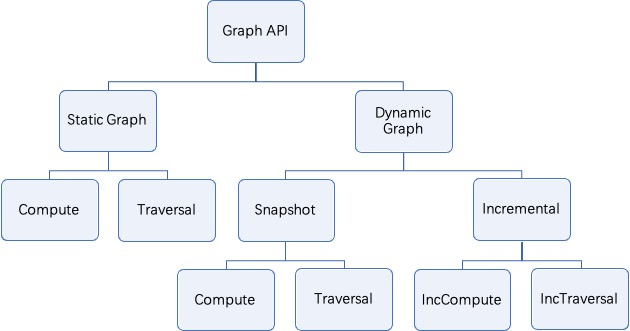
\includegraphics[width=0.95\textwidth]{./figures/api_arch.jpeg}
  \end{center}
  \caption{Geaflow API 介绍}
\end{figure}
\begin{itemize}
  \item Graph API:Graph是GeaFlow框架的一等公民,当前GeaFlow框架提供了一套基于GraphView的图计算编程接口,
    包含图构建、图计算及遍历。在GeaFlow中支持Static Graph和Dynamic Graph两种类型。
  \item Static Graph API:静态图计算API,基于该类API可以进行全量的图计算或图遍历。
  \item Dynamic Graph API:动态图计算API,GeaFlow中GraphView是动态图的数据抽象,基于GraphView之上,可以进行动态图计算或图遍历。
    同时支持对Graphview生成Snapshot快照,基于Snapshot可以提供和Static Graph API一样的接口能力。
  \item Stream API:GeaFlow提供了一套通用计算的编程接口,包括source构建、流批计算及sink输出。
    在GeaFlow中支持Batch和Stream两种类型。
  \item Batch API:批计算API,基于该类API可以进行批量计算。
  \item Stream API:流计算API,GeaFlow中StreamView是动态流的数据抽象,基于StreamView之上,可以进行流计算。
\end{itemize}

通过两种类型API的介绍可以看到,GeaFlow内部通过View统一了图视图和流视图语义。
同时为了统一支持动态和静态计算两套API,GeaFlow内部抽象了Window的概念,
即从Source API开始就必须带有Window,用以基于Window的方式切分数据窗口。

\begin{itemize}
  \item 对流或动态图API来说,Window可以按照 size 来切分,每个窗口读取一定size的数据,从而实现流式增量的计算。
  \item 对批或静态图API来说,Window将采用AllWindow模式,一个窗口将读取全量数据,从而实现全量的计算。
\end{itemize}

本文主要使用 Geaflow API 的 Graph API, Graph API是GeaFlow中的一等公民,其提供了一套基于GraphView的图计算编程接口,包含图构建、图计算及遍历。
关于 Stream API 的详细内容可参见 GeaFlow 官网\cite{ref1}.

\subsection{Graph API}
静态图:
\begin{table}[H]
  \caption{静态图}
  \begin{center}
    \begin{tabularx}{\textwidth}{Xl}
      \toprule
      \textbf{API} & \textbf{说明} \\
      \midrule
      \texttt{PGraphCompute compute(VertexCentricCompute vertexCentricCompute)} & 在Graph上进行静态图VC计算 \\
      \texttt{PGraphWindow compute(ScatterGatherCompute sgAlgorithm, int parallelism)} & 在Graph上进行静态图SG计算 \\
      \texttt{PWindowStream getEdges()} & 返回edge集合 \\
      \texttt{PWindowStream getVertices()} & 返回vertex集合 \\
      \bottomrule
    \end{tabularx}
  \end{center}
\end{table}

\subsubsection{Compute API 介绍}
GeaFlow对外提供了实现图计算算法的接口,通过实现相应接口可进行静态图计算或动态图计算,用户可在compute算法中定义具体的计算逻辑及迭代最大次数。

本文主要使用 Geaflow 的静态图接口.

静态图接口:
\begin{table}[H]
  \caption{静态图接口}
  \begin{center}
    \begin{tabularx}{\textwidth}{XlX}
      \toprule
      \textbf{API} & \textbf{接口说明} & \textbf{入参说明} \\
      \midrule
      \texttt{void init(\newline VertexCentricComputeFuncContext vertexCentricFuncContext)}
                   & 迭代计算初始化接口
                   & vertexCentricFuncContext: 静态图计算的上下文, K 表示 vertex
                   id 的类型,VV 表示 vertex value 类型,EV 表示 edge
                   value 类型,M 表示发送消息的类型。 \\
      \texttt{void compute(K vertexId, Iterator messageIterator)}
                   & 迭代计算接口
                   & vertexId: 当前计算点 id, 其中 K 表示 vertexId 的类型。
                   messageIterator: 迭代过程中所有发送给当前点的消息,
                   M 表示迭代计算过程中定义的发送消息类型。 \\
      \texttt{void finish()}
                   & 迭代计算完成接口
                   & - \\
      \bottomrule
    \end{tabularx}
  \end{center}
\end{table}

详细接口:
\begin{center}
\begin{minted}[xleftmargin=5mm]{java}
public interface VertexCentricComputeFunction<K, VV, EV, M>
  extends VertexCentricFunction<K, VV, EV, M> {
  void init(VertexCentricComputeFuncContext<K, VV, EV, M> vertexCentricFuncContext);
  void compute(K vertex, Iterator<M> messageIterator);
  void finish();

  interface VertexCentricComputeFuncContext<K, VV, EV, M>
    extends VertexCentricFuncContext<K, VV, EV, M> {
      /* 设置vertex value */
      void setNewVertexValue(VV value);
  }
}
\end{minted}
\end{center}
